\section{Background and Related Work}\label{sec-background}


\begin{figure}[htbp]
\begin{minipage}[t]{0.35\textwidth}
\centering
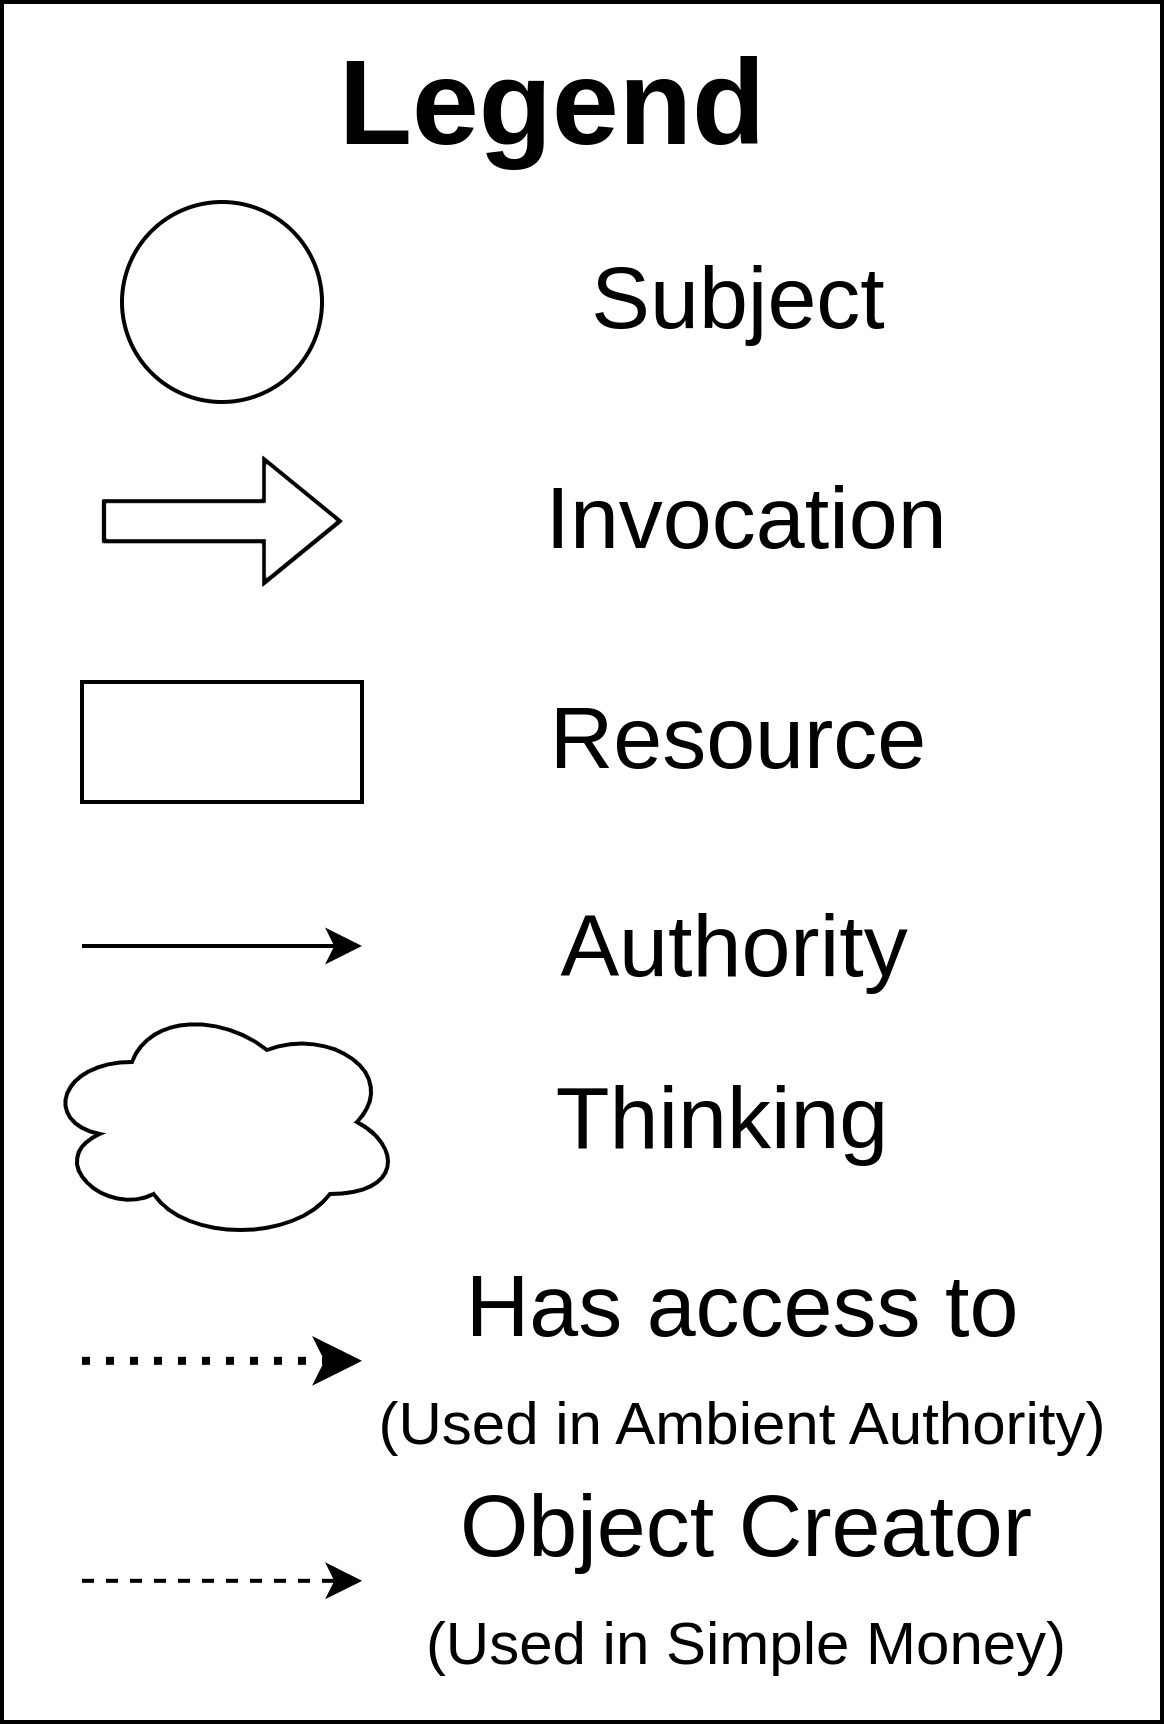
\includegraphics[width=1.4in]{figures/Legend.jpg}
\caption{Legend for various entities in object-capability diagrams}
\end{minipage}
\hspace{\fill}
\begin{minipage}[t]{0.55\textwidth}
\centering
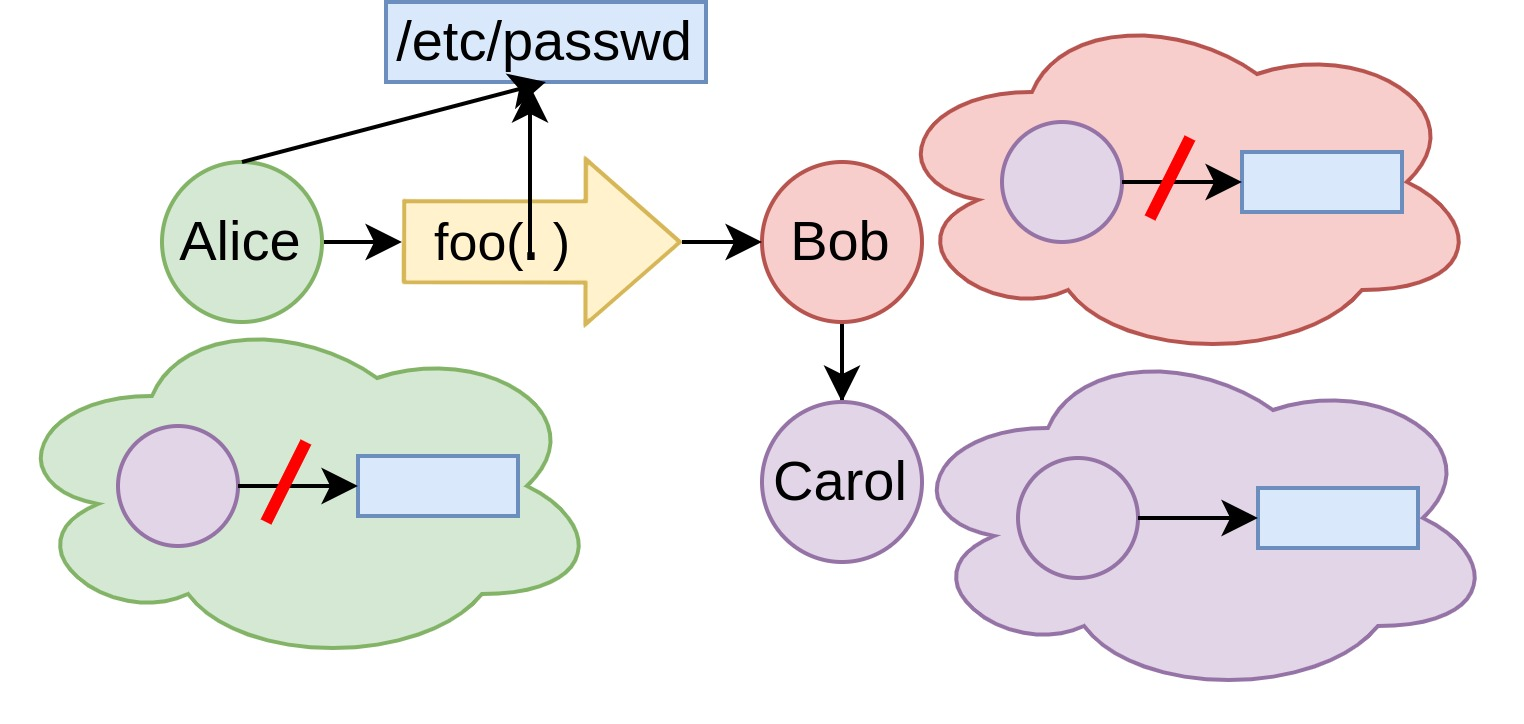
\includegraphics[width=2.8in]{figures/confused_deputy.jpg}
\caption{The Confused Deputy Problem represented as a Granovetter Diagram \cite{millerCapRights}}
\label{cdp}
\end{minipage}
\end{figure}
\noindent
We provide a background on the motivation for using capability-based design and a sample capability pattern used in one of the study designs. 

\subsection{Capabilities: Motivation}
% http://www.cap-lore.com/CapTheory/ConfusedDeputyM.html

\noindent
To start with why we need capabilities, we first need to look at the Confused deputy problem~\cite{millerCapRights}. In Figure \ref{cdp}, Bob acts as the deputy and is deemed trustworthy by every other entity (hence the term ``deputy''). He is communicating with Alice and Carol. Alice then provides Bob with a sensitive resource (in this case \texttt{/etc/passwd} with specific permissions) and trusts Bob enough not to pass the sensitive resource to Carol. The question then arises whether Carol can "trick" Bob into access to the underlying resource, thus leading to broken access control. Currently, many real-world vulnerabilities are present in this class (due to ambient authority) with common examples being Cross-Site Request Forgery (CSRF) \cite{blatz2007csrf} and VSCode extensions (\cite{vscodevuln}).

However, Rust provides module systems that don't have ambient authority, for which one could argue that these bugs would not happen in the future (i.e., we consider Bob won't be pinned as a reason for broken access control). This further propagates the question of whether capabilities as a language design choice by itself provide additional advantages.

\cite{millerCapRights} further discusses object-capabilities security as one of the methods to avoid the confused deputy problem. Capabilities can be viewed as one of the interpretations of the Granovotter diagram. It is defined as the following:

If Bob does not have access to Carol (which is a critical resource), he can only gather access to it from someone else. Let us assume it's Alice; she can only give the resource to Bob only if:
\begin{itemize}
    \item Alice already has the authority to Carol object (via a reference)
    \item Alice has a reference to Bob
    \item (Key part) Alice decides to voluntarily share the reference to Carol with Bob
\end{itemize}

% A brief overview of capabilities is given in the next section.
% Let us use this analogy in implementing the Linux operating system, where access to files is stored in an Access Control List (ACL). If (a) the running process is Bob, (b) Alice has already provided Bob with the necessary permissions to read/write the resource, and (c) Carol has already invoked Bob and is asking for the underlying resource, the underlying OS will only look at the process id of the caller, i.e., Bob, see that it has the necessary permissions, and ultimately return the result to Carol. Here, there exists ambient authority on the \texttt{/etc/passwd}, since one only needs to name the resource and the necessary operation to the right person. 


% https://wiki.c2.com/?ConfusedDeputyProblem
% One could pin the underlying reason onto Bob, saying that its methods called from Carol did not check for the authority itself and thus invoked a security hole. Even though this is true on a high level, considering that the amount of software being written is large, which would lead to more unforced errors, we need to "find a more fundamental cause." Here, the reason is that there is a separation of (a) the underlying reason for Bob's permission and (b) What Bob is actually doing.


% \begin{figure}[htbp]
% \centering
% 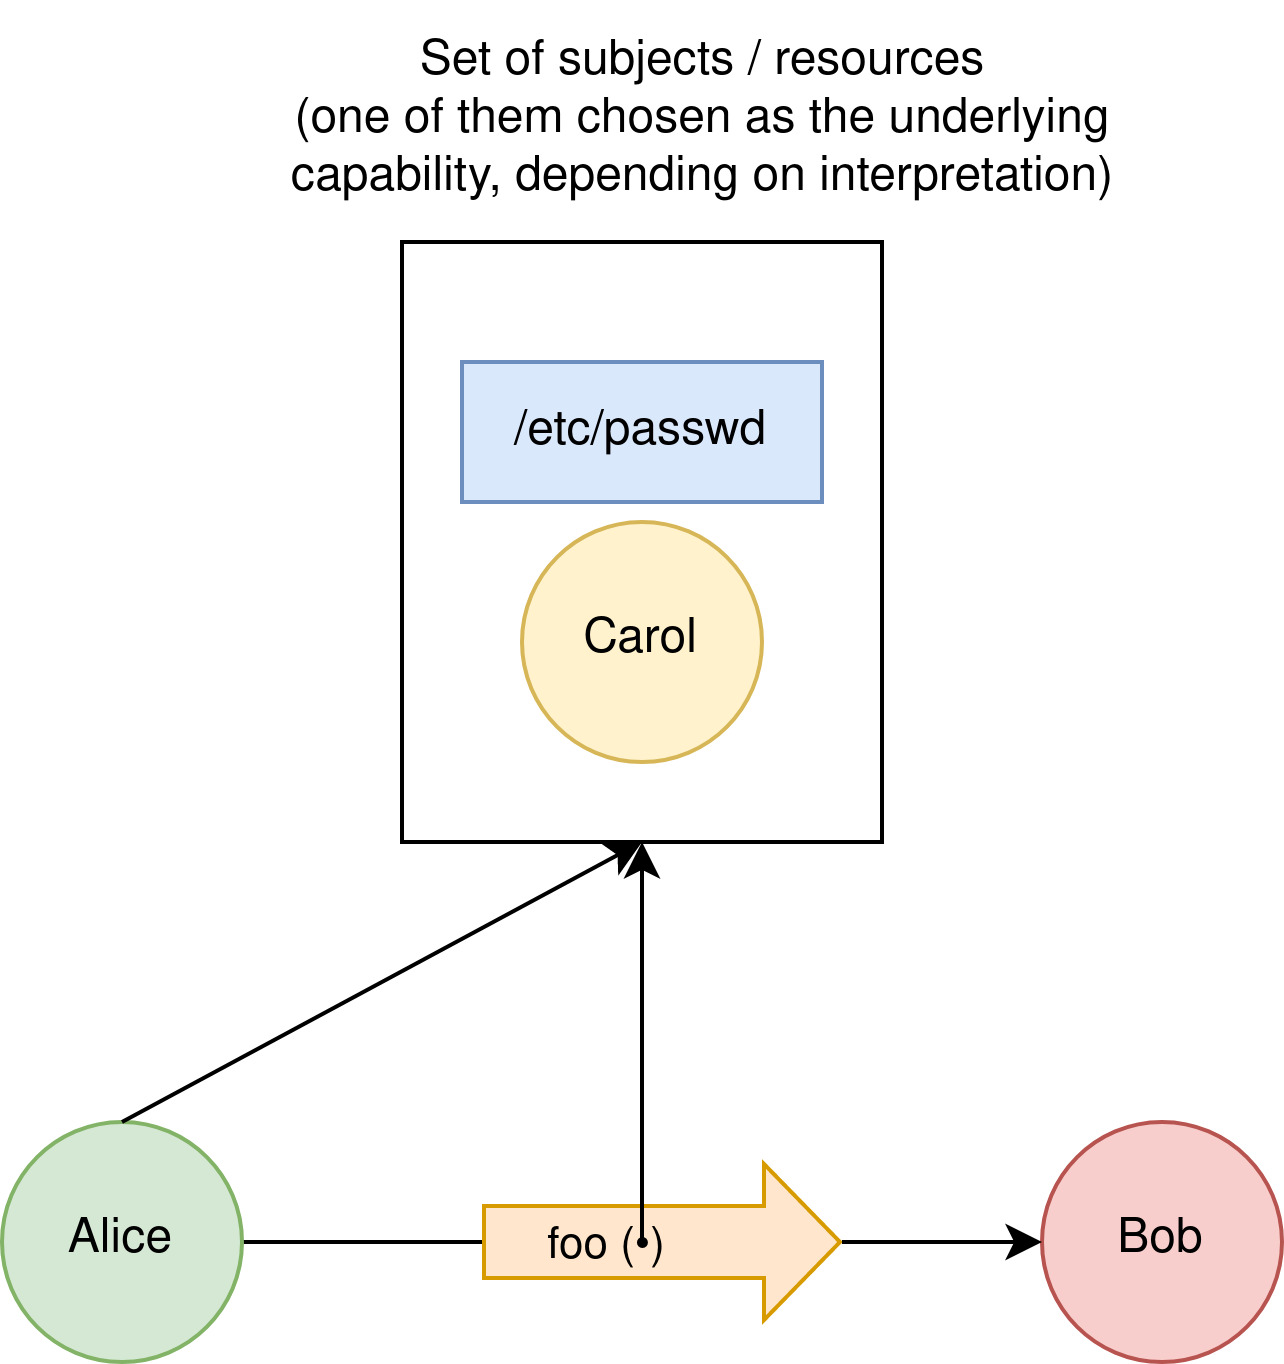
\includegraphics[width=2.5in]{figures/cap.jpg}
% \caption{The Granovetter Diagram viewed as a capability object}
% \end{figure}
% http://erights.org/elib/capability/ode/overview.html

% http://habitatchronicles.com/2017/05/what-are-capabilities/
Capabilities can be summarised as - "Don't separate authority from designation." \cite{markCapsMyth}. The design choice in creating programs with capabilities is for a main trusted program to provide the correct amount of capability (which is implemented as non-forgeable references) to each specific object.  

% Figure \ref{cap_acl} provides a shift in perspective from ACLs to capabilities.

% \begin{figure}[htbp]
% \centering
% 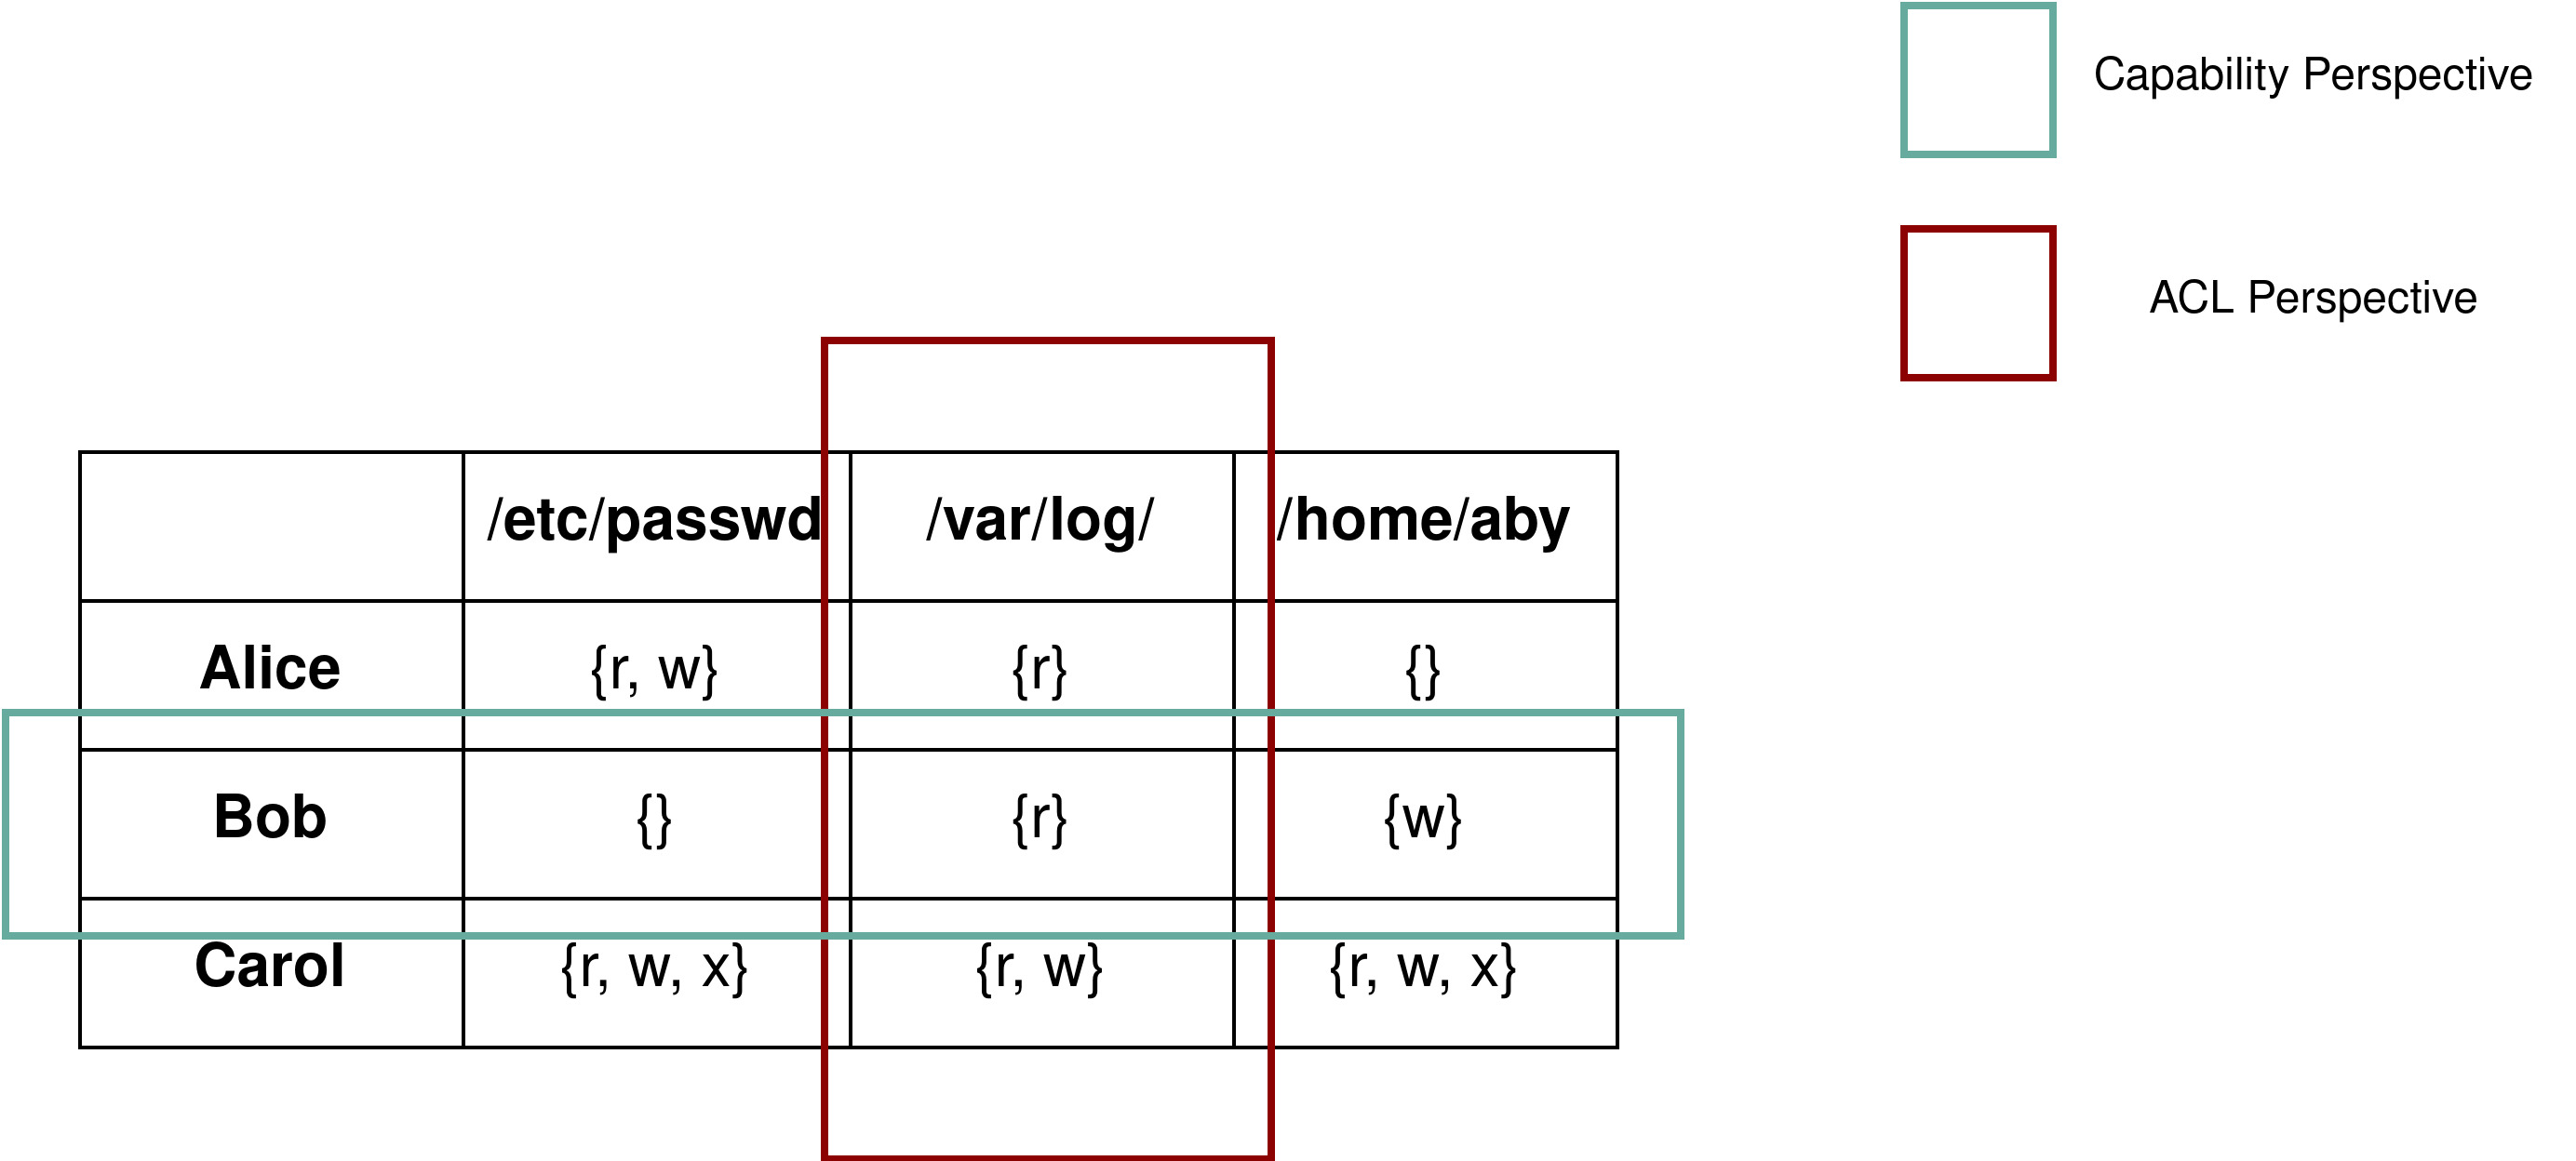
\includegraphics[width=4.0in]{figures/cap_def.jpg}
% \caption{Comparison between ACLs and Capabilities}
% \label{cap_acl}
% \end{figure}

% Here, the authority is defined from a subset of \( {r, w, x} \), which means read, write, and execute on a specific file, respectively. We can see that rows are represented with capabilities for a specific object, and columns are represented as ACLs. Now, this makes a difference in terms of who is bounded to the specific authority (represented with a cell in the table). 

% In ACLs, the resources are bound to the authority, whereas in the capabilities models, it is bound to the specific object. Now, 

\subsection{Capability Patterns: Sealer-Unsealer}

\noindent
According to \cite{millerFinancial}, sealer/unsealer pairs (Figure \ref{fig:sealerUnsealerDef}) can be conceptually viewed as similar to public/private key pairs. They can be used to control rights to access a certain object as follows:
\begin{enumerate}
    \item \textbf{Initialisation} The main program creates the sealer/unsealer pair, and passes it to Alice.
    \item \textbf{Sealing the resource} Alice invokes \texttt{seal} from a sealer object. Internally, \texttt{Sealer} creates a Sealed box, and returns it to Alice. This is represented by steps (1)-(3) in Figure \ref{fig:sealerUnsealerDef}. Considering that Alice only has access to the Sealed Box, she can pass it around without having to worry about others accessing the critical resource.
    \item \textbf{Unsealing the resource} However, Alice must be careful with passing the Unsealer around. If she passes it to another entity (this is acceptable within the design of the language since behavior is defined in trusted code, and not at runtime), they now have the ability to call unseal and gain access to the inner object. This is represented by steps (4)-(6) in Figure \ref{fig:sealerUnsealerDef}. 
\end{enumerate}

This  pattern will be used in the study design of Simple Money, which is given in section \ref{sec:simpleMoney}.

\begin{figure}[htbp]
\centering
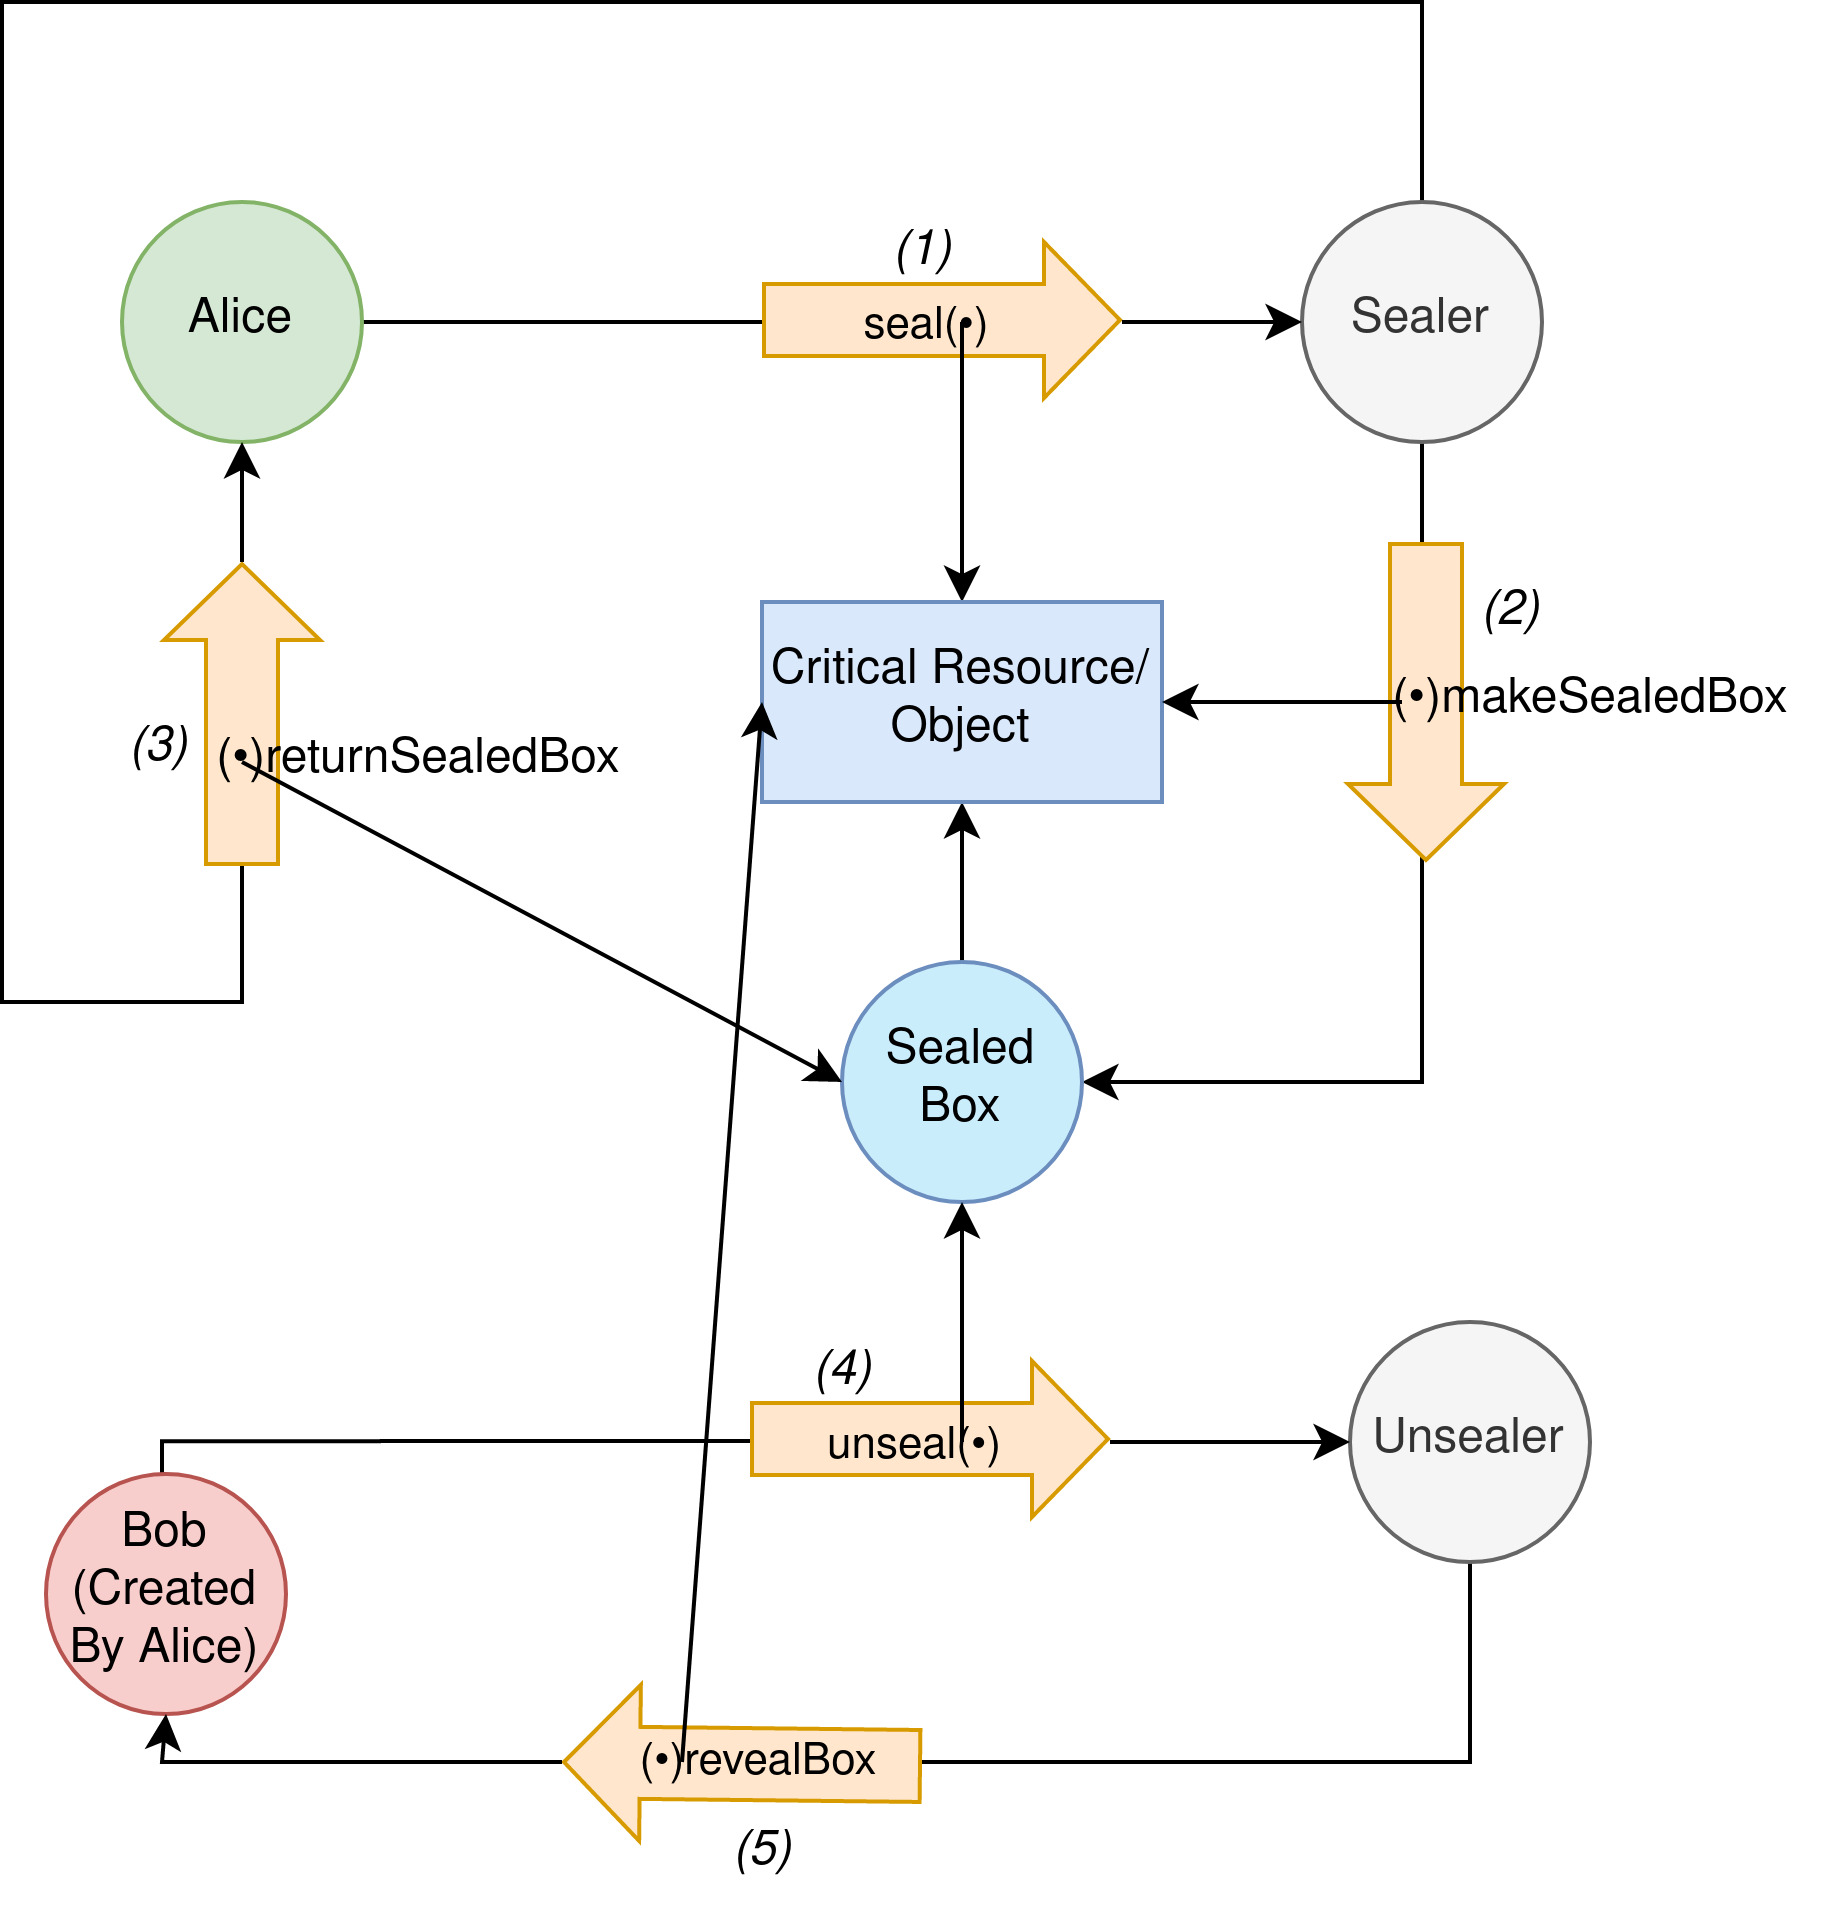
\includegraphics[width=2.5in]{figures/sealerUnsealer_def.jpg}
\caption{Sealer-Unsealer Architecture}
\label{fig:sealerUnsealerDef}
\end{figure}
% \section{Programming Languages}
% \subsubsection{Wyvern}
% \subsubsection{Rust}
